\documentclass[a4paper,10.5pt]{article}
\usepackage{amsmath,amsfonts,amsthm,bm,listings,graphicx,float,subcaption,multicol,wrapfig,stfloats}
\usepackage[export]{adjustbox}
\usepackage[labelfont=bf]{caption}
\usepackage[margin=1.1in]{geometry}
\graphicspath{ {/Users/ianmcwilliam/Desktop/MSc/Active_Learning/Tex} }
\usepackage{titling}
\setlength{\droptitle}{0cm}

\begin{document}
\title{Informatics Project Proposal - Automatic Curriculum Learning for Deep Models Using Active Learning}
\author{Ian McWilliam s0904776}
\date{}
\maketitle

\begin{abstract}
In this paper we propose a project researching how active learning methods can be used to automatically construct training curricula, with the aim being to test the hypothesis that training deep models with such `active curricula' can improve upon other training paradigms such as uniform random sampling, pre-training or traditional curriculum learning. The work will investigate a variety of methodologies for constructing a curriculum using active learning metrics, focusing on how the different training methods affect the performance of convolutional networks on a range of image classification tasks. The output of the project will hopefully be a set of novel ways to improve the training of deep models, as well as a more thorough exploration of the relationship between active and curriculum learning than currently exists in the literature.
\end{abstract}

\newpage

\section{Introduction}

\subsection*{Active Learning}
\textit{Active learning} refers to a learning paradigm wherein machine learning algorithms actively select, or `query', the samples from which it learns; in the case of deep learning this contrasts with the usual approach of uniformly sampling labeled training samples. The motivation for active learning is that, by allowing it to intelligently select the samples from which it learns, the algorithm can achieve superior generalization performance from a smaller number of training samples than if the samples had been chosen randomly. In domains where unlabeled data is abundant but obtaining labels is expensive, active learning can be used to reduce the cost associated with training a deep model, as the active approach allows the designer to obtain labels only for the samples which will be most beneficial to learning.

There are a variety of methods by which the algorithm can query datapoints, however they generally focus on finding the points in the input space that the algorithm is most `uncertain' about, allowing the algorithm to fill what could be seen as gaps in its knowledge of the domain. We can broadly categorize four main active learning approaches as follows:
\begin{itemize}
\item Uncertainty Sampling - How uncertain
\item Query by Committee (QBC) - Disagreement
\item Expected Model Change - Gradient change
\item Variance Reduction - equation etc for proof for logistic regression
\end{itemize}
We also note the work of Gal et al \cite{Gal 2016 2} who use the uncertainty inherent in Bayesian deep models, estimated by approximating variational inference with Monte Carlo dropout methods.

DISCUSS WORK OF COHN SHOWING IMPROVED GENERALIZATION PERFORMANCE?

\subsection*{Curriculum Learning}
A related field is that of \textit{curriculum learning}, which explores how the learning process can be improved by presenting training samples to the algorithm in a meaningful order (with the order defining a `curriculum'), again in contrast to simply sampling randomly from a training set. Motivated by the way in which humans and animals learn, a curriculum generally begins with `easy' examples, before transitioning to more challenging ones, with the aim being to improve generalization performance and convergence speed. TALK ABOUT BENGIO PAPER ETC. It is interesting to note that, while similar, active and curriculum learning are somewhat opposed in their learning philosophies, with the former focusing on learning from uncertain/difficult samples and the latter focusing beginning with easy samples before continuing to more difficult ones. 

Bengio et al \cite{Bengio 09} find a theoretical motivation for curriculum learning by suggesting that it can be seen as a \textit{continuation method} (a method of optimization non-convex functions). Curriculum learning has also drawn similarities with \textit{transfer learning}, as the early, `easier' stages of training can be seen as a separate task, with the network weights then being used as the initial weights for training on the more difficult samples. Similarly curriculum learning can be seen as a form of pre-training, comparing the method to unsupervised pre-training methods as in \cite{Erhan 09}, where pre-training allows the supervised learning to begin in a region of parameter space that led to superior generalization performance. 

\section{Purpose}
\subsection*{Curriculum Construction}
One of the main difficulties with implementing curriculum learning is that the curriculum must be constructed prior to training, requiring some predefined measure of difficulty with which to order the training samples. In certain domains  there may be a natural ordering of difficulty, for example in the geometric shapes example in \cite{Bengio 09}, however in many tasks manually constructing a curriculum is not as straight forward. This motivates the development of methods to automatically construct learning curricula without requiring expert domain knowledge; in this paper we suggest that using active learning metrics may be used to automatically construct such curricula, potentially providing an efficient way to improve the training of deep learning algorithms.

\subsection*{Active Curricula}
Active learning methodologies generally involve calculating a measure of the algorithm's `uncertainty' in predicting the label of a given input sample. In the traditional active learning setting, the algorithm then queries the label of the sample(s) about which it has the most uncertainty and is then trained using the selected sample(s). An alternative approach is to view the uncertainty measure as a way of approximating the `difficulty' of a given input sample, which can then be used to construct a learning curriculum, which we term an `active curriculum'.

As discussed in the introduction, active and curriculum learning offer a somewhat dichotomous view on how best to order training samples (for example Kumar et al \cite{Koller 2010} refer to active learning as being an ``anti-curriculum'' method). In active learning the samples about which the algorithm is most uncertain are chosen to train on, while in curriculum learning training focuses on training on easier samples, before progressing to more difficult ones. This trade off is one that has not been explored in the literature, and it is a dimension on which we will focus in the proposed work. 

Given an uncertainty/difficulty metric using active learning methods, we have the option of constructing a curriculum beginning with training on the least uncertain samples, or alternatively training on the sa 

\section{Background}
There have been several works that have explored the area of automating the process of constructing learning curricula, as well as similar studies which evaluate methods by which training can be improved by deviating from the usual paradigm of uniform sampling; we introduce a few of these methods here.
\subsection*{Self Paced Learning}
In the paper ``Self-Paced Learning for Latent Variable Models'', M.Pawan Kumar, B. Packar and D.Koller, 2010 \cite{Koller 2010} introduce the concept of \textit{self-paced learning} wherein, after an initial training period, a learning algorithm is trained beginning with the ``easiest'' samples. The algorithm explored in the paper is the latent SSVM model, as such, ``easiness'' in the paper is defined is calculated from how far from the separating hyperplane a training example is, analogous to the classification threshold method discussed previously. The number of samples used for training is decided by difficulty threshold, which is annealed throughout training until all samples are considered, resulting in a learning curriculum that begins with easy samples and progresses to uniformly considering all training examples. The authors test their methods on datasets from a variety of domains, specifically ``natural language processing, biology and computer vision'', illustrating that their method outperforms their benchmark. The work is an interesting example of automatically constructing a curriculum but is limited to only considering the latent SSVM model.
\subsection*{Automated Curriculum Learning for Neural Networks}
The paper ``Automated Curriculum Learning for Neural Networks'' by Graves et al, 2017 \cite{Graves 2017} focus on automatically constructing curricula for neural networks, focusing on deep models. The paper considers the problem wherein learning can be split up into a series of ``tasks'', with the goal being either to maximise performance on all tasks, or only seeking to maximise performance on a final, ``target task''. In order to do this the authors use a reinforcement learning approach by modeling an $N$-task curriculum as an $N$-arm bandit problem \cite{Bubeck 2012}, such that the reinforcement learning actions are selecting from which task to sample training examples. 

The constructed algorithm is termed ``Intrinsically Motivated Curriculum Learning'', with the reward signal being calculated from a variety of progress based measures, split into ``loss-driven progress'' and ``complexity-driven progress''. Somewhat similar to the previously outlined expected model change, loss-driven progress compares the overall loss of a model before and after training on a sample $x$ (in the paper a sample $x$ refers to a batch of input-target pairs, i.e. it is assumed that all labels are known). The other, more novel, class of reward signals considered are complexity-driven progress signals, which measure changes in the complexity of the network. The rationale behind the complexity methods is derived from the Minimum Description Length (MDL) principle, which suggests that the model complexity should increase most when trained on samples from which it is best able to generalize; training examples that drive the largest increase in model complexity are therefore chosen for training. In order to model the increase the model complexity the authors use several approaches; one is to use stochastic variational inference \cite{Kingma 2015} in order to calculate the change in the KL-Divergence between a posterior over the network weights and a fixed or adaptive prior, defining the Variational complexity gain (VCG):
\begin{equation}
V_{VCG} := KL(P_{\phi^{\prime}} || Q_{\psi^{\prime}}) - KL(P_{\phi} || Q_{\psi})
\end{equation}
where $P_{\prime{\phi}}$ and $(P_{\phi}$ are the variational posterior of the weights before and after training on a sample, and similarly for the prior $Q_{\psi}$. A simpler and quicker way to measure the change in complexity is to measure the change in the regularization term of the model loss function, assuming that the loss function is regularized. While simpler to calculate, the L2 gain method generally resulted in poor performance on the tested tasks, often under-performing uniform sampling. 

The authors test their methods by training LSTM networks on several NLP datasets, with varied results; some methods outperform uniform sampling, however many methods fail to do so across the different datasets. This work represents a similar goal to that of this paper, automatically constructing curricula for deep models, and presents several novel approaches for selecting training samples that could be adapted into active learning acquisition functions. The paper focuses solely on LSTM models however, and is limited to datasets where there is a set delineation between ``tasks''. The use of reinforcement learning to construct the curriculum is also novel, and it is interesting to note that the final policies generally resulted in an easy to hard curriculum, with the algorithm autonomously discovering implicit orderings in task difficulty and finding that it is best to begin with easier tasks, supporting the curriculum learning rationale in \cite{Bengio 09}.

\subsection*{Active Bias}
A recent paper by Chang et al, 2018 \cite{Chang 18} conducts similar experiments to the proposed approach, constructing curricula by adapting the sampling probability proportionally to two metrics, specifically classification threshold proximity and prediction variance. They test their methods for training deep models on a variety of datasets, highlighting how their methods can reduce model bias in noisy environments, as illustrated in Figure 2 of \cite{Chang 18}. The authors test their training methods on a variety of datasets, including image classification and NLP tasks, showing that consistent out-performance of their methods against a benchmark of uniform random sampling. The authors also explore whether or not selecting 'easier' or 'harder' samples lead to better results, concluding that the answer is task dependent; in easier tasks they find that it is beneficial to train on samples that the model is more uncertain about, and vice versa for more difficult, noisier problems. 

The paper is limited in that it considers a relatively limited range of uncertainty metrics and curriculum constriction methods, as well as benchmark comparisons. It would also be interesting to explore how to automatically adjust the preference for harder or easier samples throughout training in order to obtain an optimal solution, as it may be difficult to know beforehand which curriculum method will perform the best. 
\vspace{0.5cm}

While these prior works have explored methods for automatically building learning curricula, we believe the work proposed in this paper presents a novel direction for several reasons. The above papers either follow the active learning philosophy of emphasizing `uncertain'/`difficult' training samples, or the curriculum learning approach of emphasizing `easier' samples, before moving uniformly sampling; we have not however found a study thoroughly comparing the either approach, nor one that attempts to blend the two approaches for an optimal solution, as we propose to do in this paper. Prior works also generally only compare their methods to relatively simple optimization procedures, for example vanilla SGD or variants thereof. As is explained by Bengio et al in \cite{Bengio 09}, curriculum learning can be compared to pre-training or transfer learning, suggesting that they should also be benchmarks against which the performance of such methods are measured, something which the proposed work will do. 

\section{Methods}
We will test a variety of learning paradigms, each using a training curriculum derived from active learning metrics. Each tested method will therefore require two elements; first, the chosen active learning metric(s), and second the method in which a curriculum is then constructed using the metrics. 
\subsection*{Active Learning Metrics}


\subsection*{Curriculum Construction Methods}
The main way in which curricula will be constructed is by adjusting the probability with which training examples are sampled during training. For example, given an active learning acquisition function $\alpha(x_i,f_t)$, which maps the input sample $x_i$ and the the model at time $t$, $f_t$ to an estimation of the model uncertainty, we can sample training instances proportionally to the model's uncertainty of each sample:
\begin{equation}\label{Sampling Probability}
\Pr(s_i|f_t) = \frac{\alpha(x_i,f_t)}{\sum_{j=1}^{N}\alpha(x_j,f_t)}
\end{equation}
Where $\Pr(s_i|f_\tau)$ represents the probability that the training sample $x_i$ is sampled and $N$ is the number of samples in the training set\footnote{In the case that there is not a pre-constructed training set, and the algorithm is querying synthetic input samples, equation \ref{Sampling Probability} could be estimated with Monte Carlo sampling.}. 

An alternative method may take the opposite approach and prefer to sample `easier' examples, about which the model is more certain , in which case we would assign sampling probabilities as:
\begin{equation}
\Pr(s_i|f_t) = \frac{\alpha(x_i,f_t)^{-1}}{\sum_{j=1}^{N}\alpha(x_j,f_t)^{-1}}
\end{equation}
A further approach could be to alter the preference for `easier' or 'harder' examples as training progresses, for example preferring easier examples at the start of training before progressing to sampling more uncertain ones later on in training, this can be achieved by setting the sampling probability by
\begin{equation}
\Pr(s_i|f_t) = \frac{\alpha(x_i,f_t)^{\beta_t}}{\sum_{j=1}^{N}\alpha(x_j,f_t)^{\beta_t}}
\end{equation}
where
\begin{equation}
\beta_t = \frac{2t}{Num\_Epochs} - 1
\end{equation}
where $Num\_Epochs$ is the number of training epochs. Note that we will start with $\beta_t = -1$ (we assume zero based indexing), corresponding to preferring to sample the least uncertain training instances, with $\beta_t \rightarrow 1$ as training progresses, leading to increased probability of sampling uncertain training examples. 


We can also use the acquisition function to alter the weight of the prediction loss of each sample as in \cite{Chang 18}. This can serve different purposes; as the training examples are no longer sampled randomly, we introduce bias into the model (REF!). By weighting the loss of each sample proportionally to the inverse of the sampling probability, we can correct for this bias; this approach is called \textit{importance sampling}. Concretely, for importance sampling, if we sample from the training data using probabilities as in equation \ref{Sampling Probability}, we can performance importance sampling by weighting the loss of sample $i$ by a the weight $w_i$, defined as follows:
\begin{equation}
w_i \propto Pr(s_i|f_t)^{-1} N_w
\end{equation}
Where $N_w$ is a normalizing constant which ensures the weights have constant unit average, so as not to alter the global learning rate, as in \cite{Chang 18}.
Alternatively we can weight the loss of each sample proportionally to the model's uncertainty (as opposed to the inverse of the model's uncertainty, as in importance sampling), in conjunction with altering the sampling probability, i.e.
\begin{equation}
w_i \propto Pr(s_i|f_t) N_w
\end{equation}


Constructing curricula with a set of Active Learning methods. 
Various curriculum constructions, select easy, select hard, easy to hard, hard to easy

\section{Evaluation}
\subsection*{Datasets}
We use the different learning methods to train several architectures on a set of image classification tasks, potentially with several different optimization methods (i.e. Stochastic Gradient Descent, AdaGrad, ADAM):
\begin{itemize}
	\item MNIST
	\item CIFAR 10
	\item CIFAR 100
	\item Geometric Shapes
\end{itemize}
\subsection*{Benchmarks}
We compare the constructed training methods to a set of benchmark alternatives -
\begin{itemize}
	\item Uniform Sampling - Sampling randomly from the training data with a uniform probability for all samples.
	\item Self-paced learning - Methodology as in \cite{Koller 2010}, excluding samples where the loss is greater than a shrinking threshold.
	\item Pre-training - Unsupervised pre-training as in REF
	\item Pre-constructed curriculum/transfer learning - For the CIFAR 100 dataset we first train a network to classify the images into their 20 super classes, before appending an additional output layer to the network and retraining to classify images into one of the 100 `fine' class labels (i.e. transfer learning). In the case of the Geometric Shapes database we train with a curriculum as in \cite{Bengio 09}, initially training on the easy `BasicShapes' dataset, consisting of the same shapes as in `GeomShapes', but with less variability in the shapes. 
\end{itemize}

We will compare the performance of the different training methodologies, measuring the classification error on a held out test set, as well as comparing how quickly the different methods converge. 


\section{Outputs}
The main output of this project will be a comparison of the proposed training methodologies to a range of benchmarks, testing whether learning with a curriculum constructed using active learning methods can reduce generalization error and convergence speeds. Should the methodologies significantly outperform the benchmark training paradigms, it could represent an innovative way to guide the training of deep models without the need to use expert domain knowledge to construct a learning curriculum prior to training. The work will also represent a more thorough experimental exploration into whether or not it is more beneficial to learn from `easy' or 'difficult' examples, or whether gradually shifting the focus throughout learning is more beneficial.

\section{Workplan}

\newpage

\begin{thebibliography}{1}
\bibitem{Allgower 1980}
E.L.Allgower and K.Georg, ``Numerical continuation methods. An introduction'', \textit{Springer-Verlag}, 1980
\bibitem{Bengio 09}
Y.Bengio, J.Louradour, R.Collobert and J.Weston, ``Curriculum Learning'', \textit{Procedures of the International Conference on Machine Learning}, 2009
\bibitem{Bubeck 2012}
S.Bubeck, N.Cesa-Bianchi, ``Regret Analysis of stochastic and nonstochastic multi-armed bandit problems'', \textit{Machine Learning}, Issue 5(1), p1-122, 2012
\bibitem{Chang 18}
H-S,Chang, E,Learned-Miller,A.McCallum, ``Active Bias: Training More Accuracy Neural Networks by Emphasizing High Variance Samples'', \textit{Advances in Neural Information Processing Systems 31}, 2018
\bibitem{Cohn 1994}
D.Cohn, L.Atlas and T.Ladner, ``Improving Generalization with Active Learning'', \textit{Machine Learning}, Issue 15, p201-221, 1994
\bibitem{Erhan 09}
D.Erhan, P.A.Manzagol, Y.Bengio, S.Bengio and P.Vincent, ``The difficulty of training deep architectures and the effect of unsupervised pre-training'', \textit{AI \& Statistics}, 2009
\bibitem{Gal 2016}
Y.Gal, R.Islam, Z.Ghahramani, ``Deep Bayesian Active Learning with Image Data'', \textit{Advances in Neural Information Processing Systems, Bayesian Deep Learning workshop}, 2016
\bibitem{Gal 2016 2}
Y.Gal, R.Islam, Z.Ghahramani, ``Dropout as a Bayesian approximation: Representing model uncertainty in deep learning'', \textit{Procedures of the International Conference on Machine Learning}, 2016
\bibitem{Graves 2017}
A.Graves, M.G.Bellemare, J.Menick, R.Munos, and K.Kavukcuoglu. ``Automated curriculum learning for neural networks'', \textit{Proc. Machine Learning Research}, 70, p1311-1320, 2017
\bibitem{Grunwald 2007}
P.D.Gr{\"u}nwald, ``The minimum description length principle'', \textit{The MIT Press}, 2007
\bibitem{Katharopoulos 2018}
A.Katharopoulos and F.Fleuret, ``Not All Samples are Created Equal: Deep Learning with Importance Sampling'', arXiv preprint, arXiv:1803.00942, 2018
\bibitem{Kingma 2015}
D.P.Kingma, T.Salimans and M.Welling, ``Variational dropout and the local reparameterization trick', \textit{Advances in Neural Information Processing Systems 28}, p2575-2583, 2015
\bibitem{Justesen 2018}
N.Justesen, S.Risi, ``Automated Curriculum Learning by Rewarding Temporally Rare Events'', arXiv preprint, arXiv:1803.0713, 2018
\bibitem{Koller 2010}
M.Pawan Kumar, B.Packer, D.Koller, ``Self-Paced Learning for Latent Variable Models'', \textit{Advances in Neural Information Processing Systems 25}, 2010
\bibitem{Own 2000}
A.Owen, Y.Zhou, ``Safe and effective importance sampling'', \textit{Journal of the American Statistical Association}, 95(449), p135-43, 2000
\bibitem{Settles 2009}
B.Settles, ``Active Learning Literature Survey'', Computer Sciences Technical Report 1648, 2009
\bibitem{Weinshall 2018}
D.Weinshall, G.Cohen, ``Curriculum Learning by Transfer Learning: Theory and Experiments with Deep Networks'', arXiv preprint, arXiv:1802.03796, 2018
\end{thebibliography}

\newpage

\appendix
\section{Example Results}
\subsection*{Methods}
To illustrate the potential results of the work we have run some preliminary tests on the \textbf{MNIST} dataset, comparing different curriculum construction methods for a given active learning acquisition method. The chosen acquisition method is \textit{average threshold closeness}:
\begin{equation}
\alpha(x_i,f_t) = \frac{1}{M}\sum_{m=1}^{M} |(P_{f_t}(\tilde{y}_m|x_i) - \frac{1}{M})|
\end{equation}
where $M$ is the number of target classes (assuming a one-hot vector embedding), and $P_{f_t}(\tilde{y}_m|x_i)$ is the softmax probability assigned to class $m$ by the model $f_t$, given the inputs $x_i$. We test four different curriculum construction methods, and compare performance against that of uniform sampling, the tested curricula are as follows:
\begin{itemize}
\item Most Uncertain (Uncertainty Wtd) - We sample training examples proportionally to their threshold closeness, as in equation \ref{Sampling Probability}, we also weight the 	prediction loss proportionally to the same.
\item Most Uncertain (Importance Sampled) - As above, however prediction losses are weighted inversely proportional to the sample uncertainty (importance sampling).
\item Least Uncertain (Uncertainty Wtd) - As with ``Most Uncertain (Uncertainty Wtd)'', but preferring less uncertain samples.
\item Least Uncertain (Importance Sampled) - As with ``Most Uncertain (Importance Sampled)'', but preferring less uncertain samples.
\end{itemize}
Using Keras, with a TensorFlow backend, we train five models (each with one of the four above curricula and one with uniform sampling), with the following architecture, hyperparameter settings and training options:
\begin{center}
\begin{tabular}{|c|c|c|c|c|}
\hline
\multicolumn{5}{|c|}{Architecture} \\
\hline
Layer & Type & Output Dim & Activation & L2 Regularization Coefficient \\
\hline
1 & Dense & 100 & ReLU & 0.0005 \\
2 & Dense & 10 & softmax & 0.0005 \\
\hline
\end{tabular}
\end{center}

\begin{center}
\begin{tabular}{|c|c|c|c|}
\hline
\multicolumn{4}{|c|}{Optimiser} \\
\hline
Method & Learning Rate & Loss Function & Extra Parameters \\
\hline
AdaGrad & 0.001 & Cross Entropy & Keras Default\\
\hline
\end{tabular}
\end{center}

\begin{center}
\begin{tabular}{|c|c|c|c|}
\hline
\multicolumn{4}{|c|}{Training Options} \\
\hline
Batch Size & Training Epochs & Validation \% & \# Burn-In Epochs \footnotemark \\
\hline
64 & 300 & 50\% & 1\\
\hline
\end{tabular}
\end{center}
\footnotetext{As in \cite{Chang 18} we train the model with uniform random sampling for a number of ``Burn-In'' epochs at the start of training.}

\newpage
\subsection*{Results}
\begin{figure}[ht]
\begin{centering}
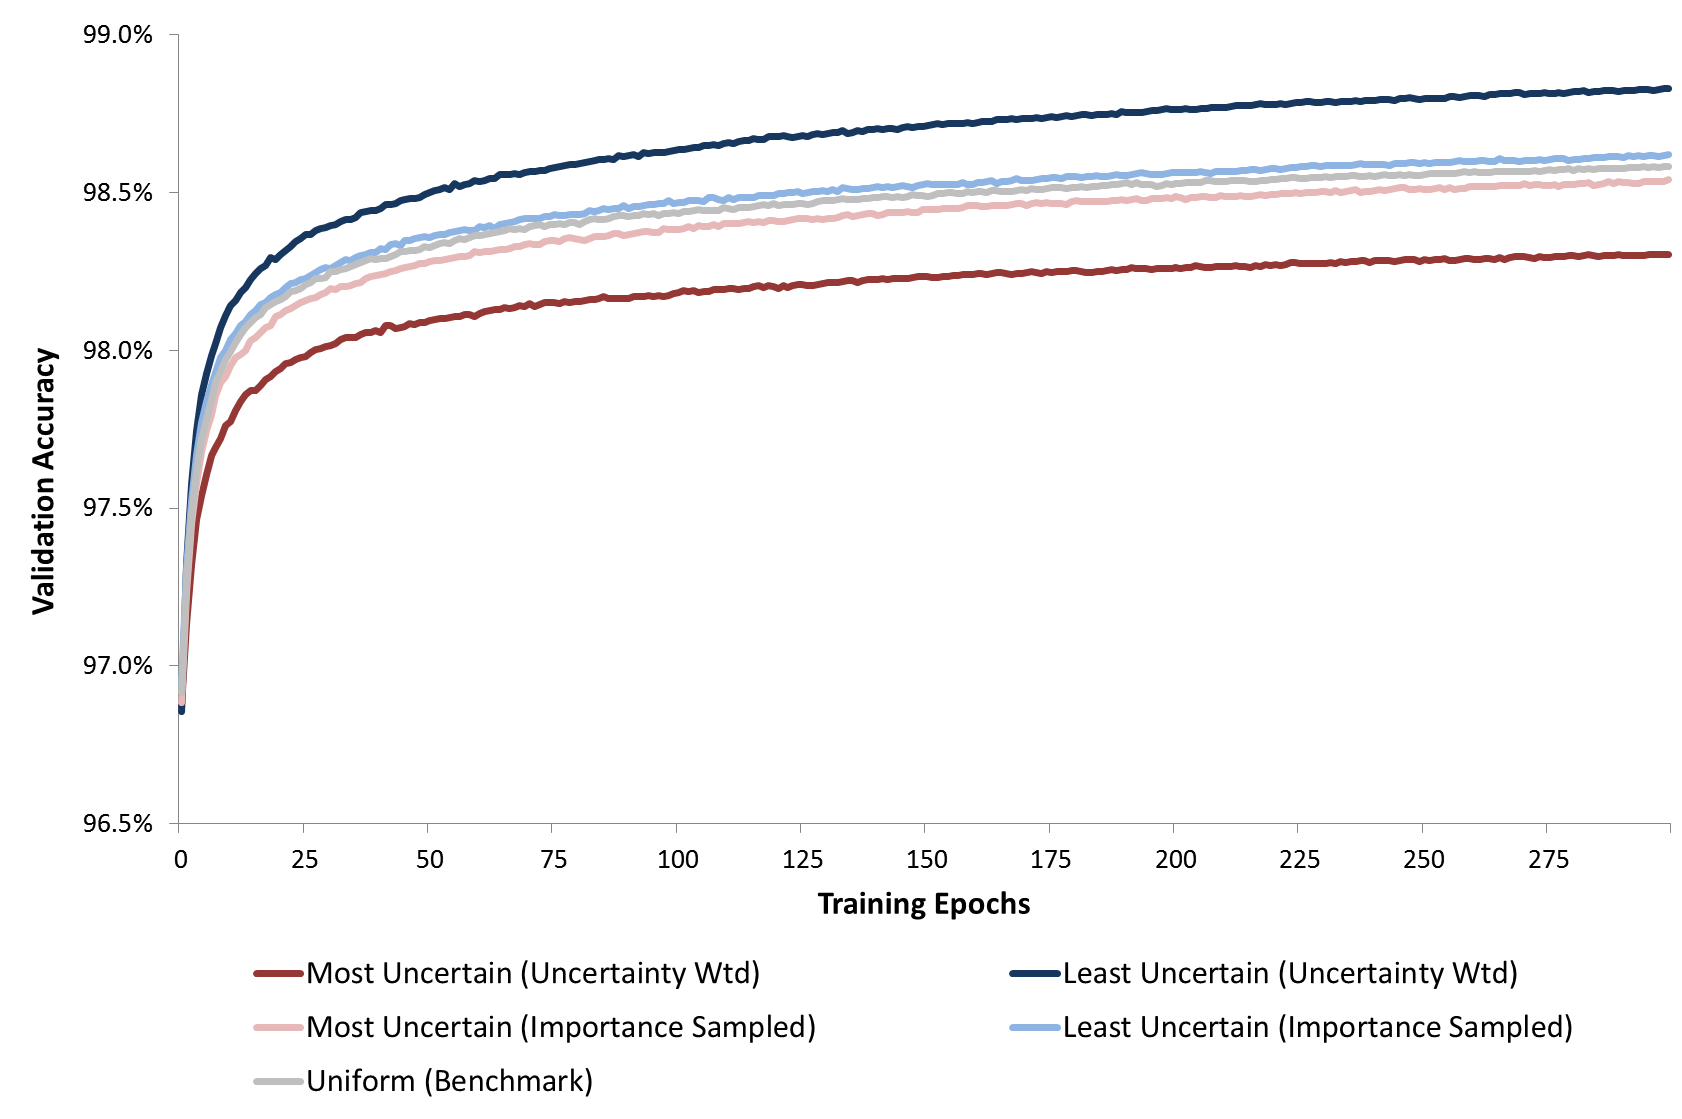
\includegraphics[scale = 0.35]{ExampleResults.png}
\caption{Validation accuracy curves for the four different learning curricula vs random uniform sampling.}
\end{centering}
\end{figure}

\begin{table}[ht]
\begin{center}
\begin{tabular}{|c|c|}
\hline
\multicolumn{2}{|c|}{Test Set Results:} \\
\hline
Curriculum &  Test Accuracy \\
\hline
Most Uncertain (Uncertainty Wtd) 		&	0.9845 \\
Most Uncertain (Importance Sampled)	& 0.9866 \\
Least Uncertain (Uncertainty Wtd) 	& \textbf{0.9891} \\
Least Uncertain (Importance Sampled)& \textbf{0.9873} \\
Uniform															& 0.9870 \\
\hline
\end{tabular}
\end{center}
\caption{Test set accuracies for trained models after 300 epochs (values in \textbf{bold} imply superior performance to uniform sampling).}
\end{table}

We see from these results that biasing sampling towards training examples about which the algorithm is \textit{least} uncertain about seems to improve test accuracy in this case, and that similarly weighting the loss function so that `easier' samples have a higher weight in the loss function also improves test accuracy. 

\end{document}